\documentclass[10pt,a4paper]{article}

\usepackage{fontspec}
\usepackage{xeCJK}
\setCJKmainfont[AutoFakeBold=2.2]{SimSun}
\setCJKsansfont[AutoFakeBold=2.2]{SimHei}
\setCJKmonofont{SimSun}
\setmainfont{Times New Roman}
\usepackage[margin=2.05cm,headheight=14pt]{geometry}
\usepackage{graphicx}
\usepackage{booktabs,array,tabularx}
\usepackage{xcolor}
\usepackage{enumitem}
\usepackage{fancyhdr}
\usepackage{caption}
\usepackage{hyperref}
\usepackage{tikz}
\usepackage{float}
\usepackage{amsmath,amssymb}
\usetikzlibrary{positioning,arrows.meta,calc}

\definecolor{ink}{RGB}{18,38,67}
\definecolor{accent}{RGB}{34,98,160}
\definecolor{soft}{RGB}{242,246,250}
\definecolor{line}{RGB}{185,196,207}
\definecolor{paperblue}{HTML}{DCEBFA}
\definecolor{papergreen}{HTML}{CFE7C1}
\definecolor{paperyellow}{HTML}{FFF0C9}
\definecolor{paperpurple}{HTML}{EADDF3}
\definecolor{dashblue}{HTML}{2474C4}
\hypersetup{hidelinks,pdftitle={Galen Context Engine Technical Report},pdfauthor={Galen Rehab Intelligence}}
\captionsetup{font=small,labelfont=bf,labelsep=quad}
\setlength{\parindent}{2em}
\setlength{\parskip}{0.26em}
\linespread{1.13}\selectfont
\newcolumntype{Y}{>{\raggedright\arraybackslash}X}
\newcommand{\Key}[1]{\textbf{#1}}
\newcommand{\Metric}[1]{{\fontsize{23}{25}\selectfont\bfseries #1}}
\newcommand{\Code}[1]{\texttt{#1}}
\renewcommand{\contentsname}{目录}
\renewcommand{\figurename}{图}
\renewcommand{\tablename}{表}

\pagestyle{fancy}
\fancyhf{}
\lhead{\small\sffamily GALEN CONTEXT ENGINE}
\rhead{\small\sffamily 技术报告 v3.0}
\cfoot{\small\thepage}
\renewcommand{\headrulewidth}{0.4pt}

\begin{document}

\begin{titlepage}
\thispagestyle{empty}
\vspace*{1.55cm}
{\sffamily\large\bfseries GALEN REHAB INTELLIGENCE\par}
\vspace{0.2cm}
\rule{\linewidth}{1.15pt}\par
\vspace{1.25cm}
{\fontsize{27}{35}\selectfont\bfseries
Galen Context Engine：\\
面向康复科研的项目状态驱动\\
上下文工程架构\par}
\vspace{0.55cm}
{\Large 技术报告\par}
\vspace{1.18cm}
\noindent\begin{minipage}{0.9\linewidth}
\large
本报告提出 Galen Context Engine：一种将研究问题、项目范围、多源 RehabID 数据、证据、工具调用与正式研究产物组织为同一可计算项目状态的上下文工程架构。系统以运动疲劳恢复研究为首个验证场景，完成从外部康复工作台接入脱敏队列、生成分析任务到交付可预览 PDF 的闭环，并以冻结任务卡对架构稳定性、工具开销与交付完成率进行验证。
\end{minipage}

\vfill
\begin{tabularx}{\linewidth}{@{}lY@{}}
\toprule
报告版本 & v3.0 \\
完成日期 & 2026 年 9 月 13 日 \\
核心对象 & Galen Context Engine 与 RehabID Connector \\
验证场景 & 运动疲劳恢复的连续科研任务 \\
\bottomrule
\end{tabularx}
\end{titlepage}

\section*{摘要}
\addcontentsline{toc}{section}{摘要}
康复科研的难点并不在于缺少一个能够生成文字的模型，而在于研究过程缺少持续可用的状态：研究范围会在讨论中修订；量表、HRV、动作表现与主观疲劳分散在不同系统；检索、分析和写作的中间结果难以进入下一步任务；最终交付常无法回到数据与决策来源。Galen Context Engine 将这些对象统一为项目状态，并以状态而非聊天长度作为连续科研任务的基础。

该架构由五类上下文构成：项目上下文、数据上下文、证据上下文、执行上下文和交互上下文。每次任务运行时，系统依据当前任务意图从有效状态中选择最小充分上下文；当用户确认新决策、切换研究范围或导入新数据时，系统写入状态事件并保留修订轨迹。Connector 负责将外部工作台的脱敏 RehabID 队列接入数据上下文；PI 对话负责提出与编排研究任务；工具层完成检索、分析、引用核验与 LaTeX/PDF 编译；所有产物回写至项目状态。

在 15 张冻结康复科研任务卡、每卡 5 次重复的受控对照中，Galen 完成 74/75 次任务（98.7\%），基线 CLI Agent 完成 21/75 次任务（28.0\%）；可观察工具调用均值为 2.11 对 6.12 次，中位端到端时延为 9.2 对 19.3 秒。独立的连续约束修订探针达到 9/9，通过范围切换探针达到 8/8；连接器演示队列包含 12 个 RehabID、48 个时间点和 204 条观察记录，并完成正式 PDF 交付。结果表明，显式项目状态、数据契约和产物验收共同构成了康复科研 Agent 可执行、可复核和可连续工作的基础。

\begin{center}
\begin{tabularx}{\linewidth}{@{}YYY@{}}
\toprule
\Metric{98.7\%} & \Metric{2.11} & \Metric{9.2 s} \\
冻结任务卡通过率 & 平均工具调用次数 & 中位端到端时延 \\
\bottomrule
\end{tabularx}
\end{center}

\tableofcontents
\newpage

\section{问题：科研任务需要项目状态，而不是更长的聊天记录}
研究者在连续科研任务中同时面对两种失败：一方面，同一项目中的样本、结局、协议和既有决定会被遗忘，研究者被迫反复解释；另一方面，项目已经改变方向后，旧病种、旧方法或旧假设仍然进入后续回答。二者本质上都是状态管理失败：前者没有持久保存有效状态，后者没有让失效状态退出当前推理。

对康复科研而言，这个问题更具体。一次观察至少应关联研究对象、采集时间、任务阶段、指标、单位、设备来源和质量标记。若 HRV、CMJ、RPE/VAS 与干预记录分别停留在不同文件或产品中，研究者无法稳定回答三个问题：\Key{某个变化发生在何时？它相对个人基线意味着什么？这一结论依据哪一组数据与证据？}

Galen 的设计目标不是扩张聊天历史，而是让研究过程中的有效对象形成可计算状态：
\begin{enumerate}[leftmargin=2.1em,itemsep=3pt]
\item \Key{连续性：}协议、样本、变量与已确认决策可以被后续任务准确继承；
\item \Key{隔离性：}研究范围修订后，旧方向退出当前推理，同时保留完整修订历史；
\item \Key{可追溯性：}数据、证据、工具调用、图表和 PDF 产物之间存在可回看的关联；
\item \Key{可执行性：}研究任务可以从数据接入一路推进到分析与正式交付，而非停留于建议文本。
\end{enumerate}

\section{方法：Galen Context Engine}
\subsection{五类上下文构成一个研究项目}
Galen 以项目为计算单位。一个项目状态并非单个 prompt，而是五类相互连接的对象：
\begin{itemize}[leftmargin=2.1em,itemsep=2pt]
\item \Key{项目上下文：}研究问题、当前有效范围、排除范围、协议约束与决策版本；
\item \Key{数据上下文：}RehabID、纵向时间点、变量、单位、质量标记与来源；
\item \Key{证据上下文：}文献条目、数据来源、检索覆盖状态与主张引用指针；
\item \Key{执行上下文：}任务节点、工具调用、输入输出、资源预算和中间产物；
\item \Key{交互上下文：}研究者确认过的结论、必要对话摘要和修订事件。
\end{itemize}

\begin{figure}[H]
\centering
\begin{tikzpicture}[font=\small,
  frame/.style={draw=dashblue, dashed, line width=0.8pt, rounded corners=2pt},
  unit/.style={draw=ink, rounded corners=2pt, minimum height=0.72cm, align=center, text width=1.67cm, inner sep=3.5pt},
  calcunit/.style={draw=ink, rounded corners=2pt, minimum height=0.85cm, align=center, fill=paperyellow, text width=2.45cm, inner sep=4pt},
  flow/.style={-{Latex[length=2.1mm]}, line width=0.72pt, draw=ink},
  feedback/.style={-{Latex[length=2.0mm]}, line width=0.72pt, draw=accent}]
  \node[frame, minimum width=6.35cm, minimum height=5.5cm, anchor=north west] (stateframe) at (0,0) {};
  \node[anchor=south west, font=\bfseries] at ([xshift=2pt,yshift=2pt]stateframe.north west) {项目状态 $S_t$};
  \node[unit, fill=papergreen] (project) at (1.18,-1.02) {项目上下文\\问题 / 范围 / 决策};
  \node[unit, fill=paperblue] (data) at (3.18,-1.02) {数据上下文\\RehabID / 时间轴 / 质量};
  \node[unit, fill=papergreen] (evidence) at (5.18,-1.02) {证据上下文\\来源 / 覆盖 / 引用};
  \node[unit, fill=paperblue] (execution) at (2.18,-2.36) {执行上下文\\任务 / 工具 / 中间产物};
  \node[unit, fill=paperpurple] (interaction) at (4.18,-2.36) {交互上下文\\确认 / 摘要 / 修订};
  \node[draw=ink, rounded corners=2pt, fill=white, minimum width=4.45cm, minimum height=0.7cm, align=center] (statevector) at (3.18,-4.06) {$S_t=\big[$ 有效范围 $\mid$ 数据资产 $\mid$ 证据指针 $\mid$ 执行记录 $\big]$};
  \foreach \n in {project,data,evidence,execution,interaction}
    \draw[flow] (\n.south) |- (statevector.north);
  \node[frame, minimum width=4.15cm, minimum height=5.5cm, anchor=north west] (engineframe) at (7.15,0) {};
  \node[anchor=south west, font=\bfseries] at ([xshift=2pt,yshift=2pt]engineframe.north west) {Galen Context Engine};
  \node[unit, fill=paperblue, text width=2.4cm] (intent) at (9.22,-0.88) {当前研究任务 $I_t$\\问题 / 目标产物 / 约束};
  \node[calcunit] (selector) at (9.22,-2.18) {有效状态选择器\\active / relevant / auditable};
  \node[calcunit] (assembler) at (9.22,-3.65) {任务上下文编排器\\按任务取最小充分状态};
  \node[draw=ink, rounded corners=2pt, fill=white, minimum width=2.78cm, minimum height=0.67cm, align=center] (packet) at (9.22,-4.65) {最小充分上下文包 $C_t$};
  \draw[flow] (intent.south) -- (selector.north);
  \draw[flow] (selector.south) -- (assembler.north);
  \draw[flow] (assembler.south) -- (packet.north);
  \draw[flow] (statevector.east) -- (selector.west |- statevector.east) |- (selector.west);
  \node[frame, minimum width=4.2cm, minimum height=5.5cm, anchor=north west] (piframe) at (12.15,0) {};
  \node[anchor=south west, font=\bfseries] at ([xshift=2pt,yshift=2pt]piframe.north west) {PI 工作回路};
  \node[calcunit, text width=2.45cm] (plan) at (14.25,-1.0) {研究计划\\提出假设 / 安排任务};
  \node[calcunit, text width=2.45cm] (tools) at (14.25,-2.45) {工具执行\\检索 / 分析 / 引用核验};
  \node[unit, fill=paperpurple, text width=2.45cm, minimum height=0.95cm] (artifact) at (14.25,-4.08) {正式研究产物\\图表 / 证据链 / LaTeX--PDF};
  \draw[flow] (packet.east) -- (plan.west);
  \draw[flow] (plan.south) -- (tools.north);
  \draw[flow] (tools.south) -- (artifact.north);
  \node[font=\scriptsize, text=accent, align=center] (eventlabel) at (11.65,-5.22) {状态事件 $e_t$\\版本 / 结论 / 产物指针};
  \draw[feedback] (artifact.south) |- (eventlabel.east);
  \draw[feedback] (eventlabel.west) -| (interaction.south);
\end{tikzpicture}
\caption{Galen Context Engine 的项目状态驱动架构。虚线框表示边界清晰的系统模块；五类上下文形成可更新的项目状态，任务上下文由状态选择器与编排器生成，PI 工作回路将研究产物以状态事件回写。}
\label{fig:architecture}
\end{figure}

\subsection{任务上下文的选择与更新}
令 $S_t$ 表示时刻 $t$ 的项目状态，$I_t$ 表示当前任务意图。系统不把全部历史直接附加给模型，而是组合当前任务所需的最小充分上下文：
\[
C_t=\operatorname{Compose}(S_t,D_t,R_t,X_t\mid I_t),
\]
其中 $D_t$ 为已纳入的数据资产，$R_t$ 为可用证据，$X_t$ 为任务与工具状态。组合过程遵守三条规则：\Key{有效优先}，仅注入 active 状态的范围和决定；\Key{任务相关}，仅取与分析、检索或交付直接相关的数据切片；\Key{历史可审计}，归档与被替换内容保留版本关系，但不进入当前任务。

新的用户确认、研究范围变更或数据导入被表示为状态事件 $e_t$：
\[
S_{t+1}=\operatorname{Apply}(S_t,e_t),\qquad H_{t+1}=H_t\cup\{e_t\}.
\]
这里 $S_{t+1}$ 直接服务下一次推理，$H_{t+1}$ 保存完整修订轨迹。这一分离使“该记住的约束被继承”与“已经退出的方向不再干扰当前任务”可以同时成立。

\section{系统：从 RehabID 接入到正式研究产物}
\subsection{统一的 RehabID 数据契约}
RehabID 是研究范围内的脱敏数据身份，不是设备编号，也不是患者姓名。最小观察记录表示为：
\[
o_i=\langle r_i,t_i,m_i,v_i,x_i,u_i,q_i,p_i\rangle,
\]
其中 $r_i$ 为 RehabID，$t_i$ 为时间点或访视，$m_i$ 为数据模态，$v_i$ 为变量，$x_i$ 为观测值，$u_i$ 为单位，$q_i$ 为质量状态，$p_i$ 为来源指针。它使“HRV 下降”可以追溯到特定对象、时点、设备记录和质量检查，而不再只是脱离来源的一句话。

\begin{table}[H]
\centering\small
\begin{tabularx}{\linewidth}{@{}c p{2.55cm} Y Y@{}}
\toprule
步骤 & 状态变化 & 关键操作 & 可观察产物 \\
\midrule
1 & 接入 & Connector 发现外部工作台的已选脱敏队列 & RehabID 列表、来源标识 \\
2 & 规范化 & CSV、JSON、量表与设备记录映射至统一字段 & 变量、单位、时间格式 \\
3 & 质检与对齐 & 检查缺失、重复、异常和时间顺序；按 RehabID 组织纵向数据 & 质量状态、个体时间轴 \\
4 & 推理与分析 & PI 任务调用数据、检索与分析工具，读取有效项目状态 & 分析结果、证据指针、修订日志 \\
5 & 交付 & 图表、方法、结果和引用被编译为正式论文 & LaTeX 源码、PDF 与预览链接 \\
\bottomrule
\end{tabularx}
\caption{Galen 的端到端执行链。每一步均将可观察结果回写为项目状态。}
\label{tab:pipeline}
\end{table}

\subsection{研究对象与产品对象分离}
工作台、可穿戴设备、力台、量表和个人端软件都不是 Galen 的研究对象本身，而是数据接入点。它们向同一个项目贡献带来源和质量标记的观察；Galen 的职责是将这些观察放入正确的研究范围与时间轴，再驱动后续分析。该设计使新增设备不需要改写研究逻辑，只需满足 RehabID 数据契约。

\begin{figure}[H]
\centering
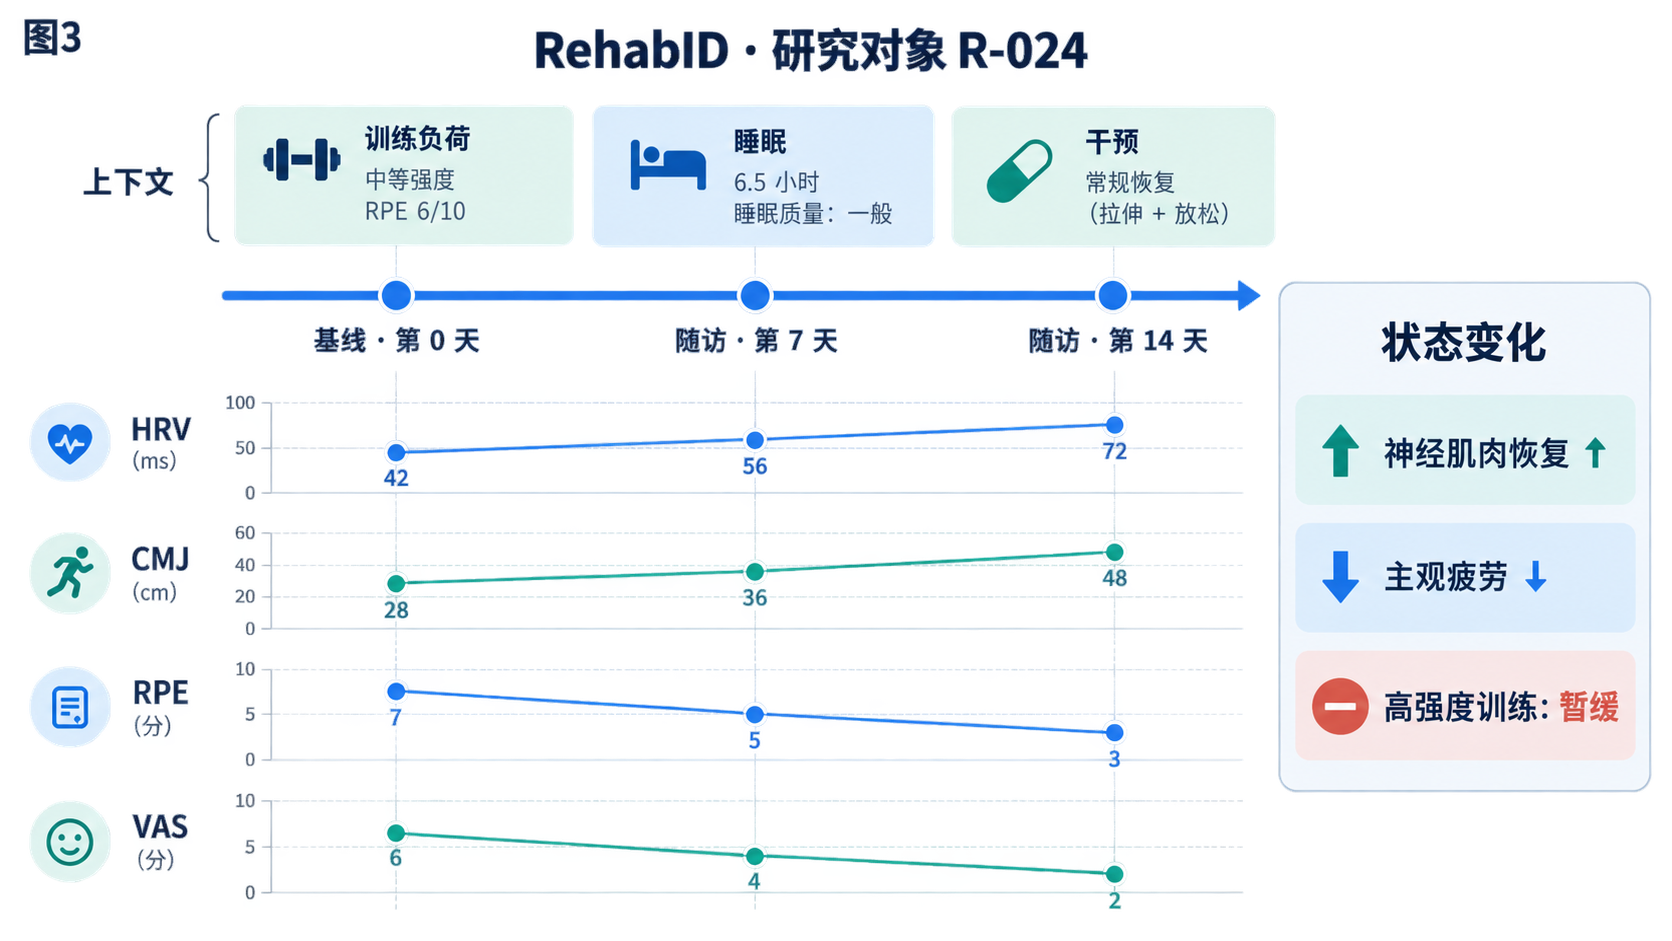
\includegraphics[width=0.9\linewidth]{assets/fig03-rehabid-timeline-zh.png}
\caption{RehabID 作为纵向研究对象，将多时间点、多指标观察统一进入项目时间轴。}
\label{fig:rehabid}
\end{figure}

\section{评测：如何验证一套上下文工程架构}
\subsection{冻结任务卡与对照条件}
评测围绕三类任务展开：上下文保持（PCTX01--05）、数据治理（PDATA01--05）和工具/交付（PTOOL01--05）。每张任务卡固定必需事实、禁用事实、必需产物、工具预算、最大模型请求次数和重复上限。Galen 与基线 CLI Agent 使用相同模型标签、相同输入和独立工作区；每张卡运行 5 次，共形成 75 组配对运行。

一次运行仅在以下条件同时满足时计为通过：进程完成；必需事实完整保留；禁用内容未进入结果；产物存在且可预览；工具顺序与调用预算满足任务卡；无重复调用环路。该口径把“回答看起来合理”转化为可检查的工作流完成标准。

\subsection{指标}
对任务 $j$，记硬门通过为 $g_j\in\{0,1\}$，工具调用数为 $n_j$，端到端时延为 $\tau_j$。报告三组核心指标：
\[
\text{PassRate}=\frac{1}{N}\sum_{j=1}^{N}g_j,\qquad
\bar{n}=\frac{1}{N}\sum_{j=1}^{N}n_j,\qquad
\widetilde{\tau}=\operatorname{median}(\tau_1,\ldots,\tau_N).
\]
同时保留约束继承、范围隔离、数据契约与产物交付的逐项断言，使整体数字可以回到失败任务类型和原始运行记录。

\section{结果：项目状态改变了任务完成方式}
\subsection{冻结任务卡上的架构对照}
\begin{table}[H]
\centering\small
\begin{tabularx}{\linewidth}{@{}YcccY@{}}
\toprule
系统 & 运行次数 & 硬门通过 & 平均工具调用 & 中位端到端时延 \\
\midrule
Galen Context Engine & 75 & \textbf{74/75 (98.7\%)} & \textbf{2.11} & \textbf{9.2 s} \\
基线 CLI Agent & 75 & 21/75 (28.0\%) & 6.12 & 19.3 s \\
\bottomrule
\end{tabularx}
\caption{在相同冻结任务卡和运行条件下的架构对照结果。}
\label{tab:main-result}
\end{table}

Galen 比基线多完成 53 次任务。差异并非来自“更少调用工具”这一孤立目标，而是来自任务启动时已拥有明确的项目状态、必需事实和产物验收条件：系统较少反复探索目录、重读无关历史或在失败后循环调用工具。图 \ref{fig:success} 与图 \ref{fig:efficiency} 展示了通过率、工具调用与端到端时延的差异。

\begin{figure}[H]
\centering

\includegraphics[width=0.88\linewidth]{assets/fig07-framework-success-zh.pdf}
\caption{冻结任务卡上的硬门通过率。}
\label{fig:success}
\end{figure}

\begin{figure}[H]
\centering

\includegraphics[width=0.88\linewidth]{assets/fig08-framework-efficiency-zh.pdf}
\caption{可观察工具调用与端到端时延。}
\label{fig:efficiency}
\end{figure}

\subsection{两类上下文核心能力}
连续约束修订探针要求系统在三轮任务中继承协议号、样本量、主要结局与工具读取事实，并将随访窗口由 12 周更新为 16 周，结果为 9/9 断言通过。运动疲劳项目接管探针要求系统在历史项目存在的前提下切换至 \Code{GALEN-FATIGUE-01}，并在不重复研究范围的情况下提出 HRV、CMJ 与 RPE 的纵向分析方案，结果为 8/8 断言通过。

\begin{table}[H]
\centering\small
\begin{tabularx}{\linewidth}{@{}p{3.65cm}Ycc@{}}
\toprule
探针 & 验收对象 & 断言结果 & 用时 \\
\midrule
连续约束修订 & 继承协议、保留工具事实、应用最新随访修订 & \textbf{9/9} & 55.998 s \\
项目范围切换 & 当前范围接管、旧方向隔离、生成纵向分析方案 & \textbf{8/8} & 33.000 s \\
\bottomrule
\end{tabularx}
\caption{Context Engine 的两类核心验证。}
\label{tab:probes}
\end{table}

\subsection{从队列到正式论文的交付闭环}
在演示队列中，Connector 导入 12 个 RehabID、48 个时间点和 204 条观察记录。数据进入项目状态后，PI 任务按队列质量检查、72 小时纵向比较和正式论文交付三个节点推进；最终生成带方法、结果、图表和引用的 LaTeX/PDF 产物。该过程将数据接入、研究任务与论文交付放在同一条可回看的执行链中。

\begin{figure}[H]
\centering
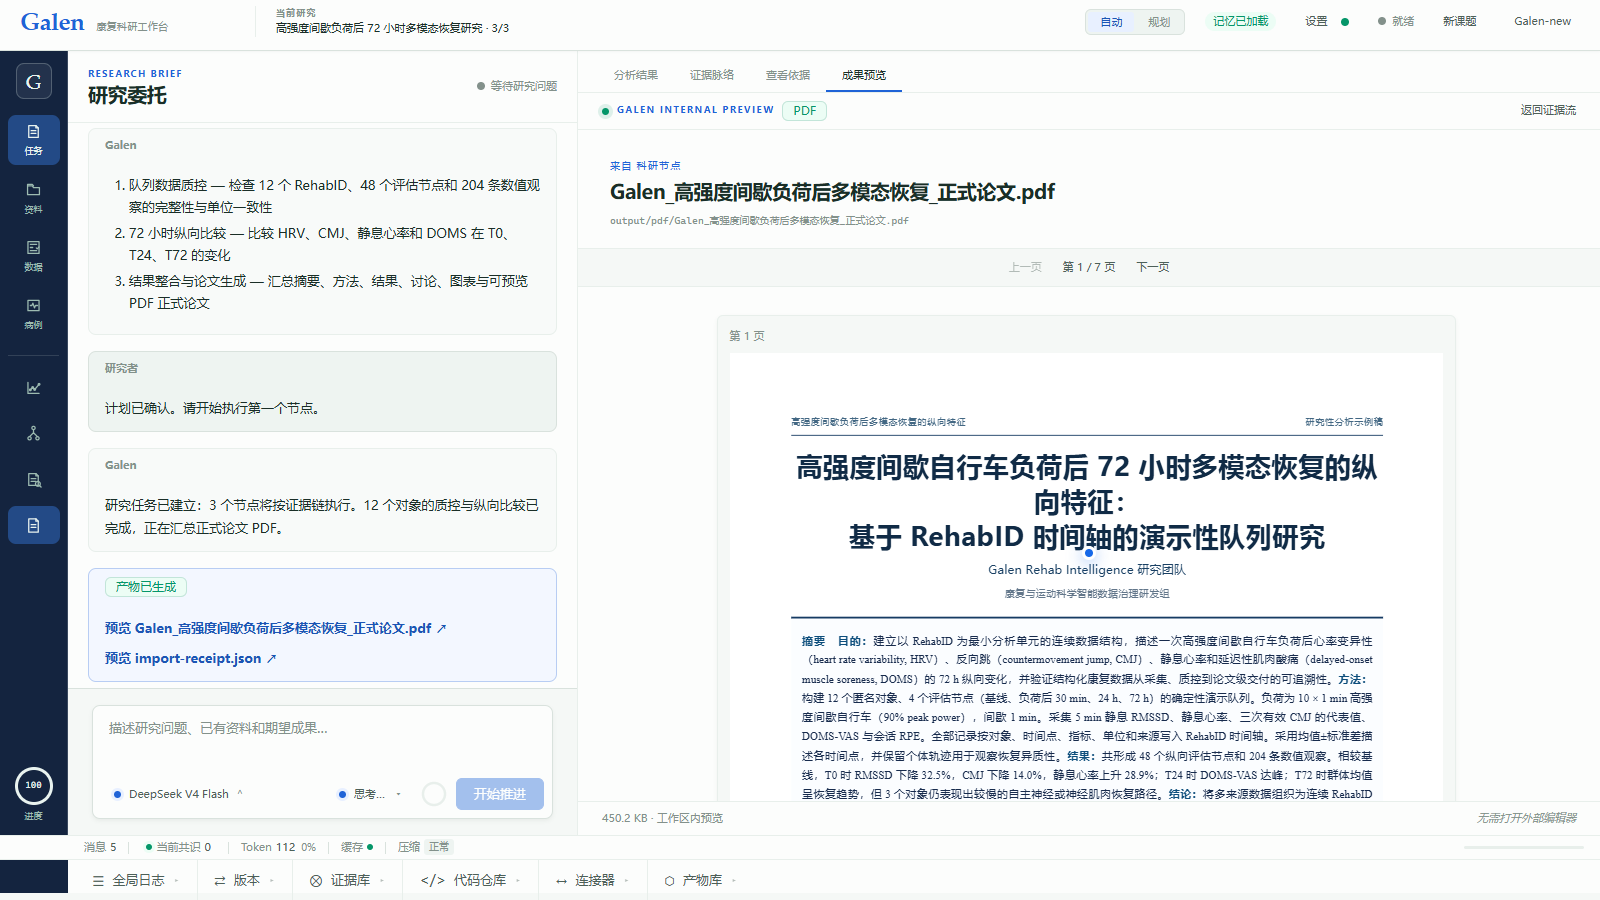
\includegraphics[width=0.94\linewidth]{assets/paper-preview.png}
\caption{Galen 工作台中的正式论文 PDF 预览。论文产物保留项目范围、任务版本和数据来源入口。}
\label{fig:paper}
\end{figure}

\section{讨论：为什么这是上下文工程，而不是检索增强聊天}
传统 RAG 主要解决“从文档中找到相关文本”；Galen 解决的是“让一个科研项目在多轮、多工具、多数据源条件下保持正确的工作状态”。二者并不冲突：文献检索结果应进入证据上下文，成为后续方案、分析和论文引用的组成部分；但检索本身不能替代项目范围、数据契约、执行节点与产物验收。

本架构的技术贡献在于把上下文从模型输入的临时拼接，提升为可更新、可审计、可执行的系统层对象。其价值可以概括为三点：\Key{一是}让研究范围有明确的 active、archived 与 revised 生命周期；\Key{二是}让异构康复数据以 RehabID 和时间轴进入同一研究对象；\Key{三是}让工具调用和正式交付留在同一条可复核的执行记录中。

\section{结论}
Galen Context Engine 提出了一种面向康复科研的项目状态驱动上下文工程架构。它以五类上下文组织研究过程，以事件驱动状态更新，以 RehabID 数据契约承接外部系统，并以工具和产物的闭环把科研任务推进到正式 PDF 交付。冻结任务卡、连续修订探针、范围切换探针和队列到论文的完整流程共同表明：当研究约束、数据、证据和执行记录围绕同一项目状态运行时，康复科研 Agent 能够以更稳定、更经济的方式完成连续任务。

\appendix
\section{可复现材料}
\begin{itemize}[leftmargin=2.1em,itemsep=2pt]
\item Context Engine 源码与测试：\Code{rust/crates/galen/}；
\item 冻结任务卡与运行记录：\Code{evals/cases/paired/}、\Code{evals/runs/}；
\item 两类上下文探针：\Code{context-memory-probe.json} 与 \Code{fatigue-scope-probe.json}；
\item 数据到论文演示视频：\Code{output/galen-promo/out/}；
\item 正式论文产物：\Code{output/real-galen-paper-run-v2/output/papers/}。
\end{itemize}

\end{document}
